\documentclass[12pt]{article}

% Imported Packages
%------------------------------------------------------------------------------
\usepackage{placeins}
\usepackage{amssymb}
\usepackage{amstext}
\usepackage{amsthm}
\usepackage{amsmath}
\usepackage{enumerate}
\usepackage{fancyhdr}
\usepackage[margin=1in]{geometry}
\usepackage{graphicx}
\usepackage{extarrows}
\usepackage{setspace}
\usepackage[utf8]{inputenc}
%------------------------------------------------------------------------------

% Header and Footer
%------------------------------------------------------------------------------
\pagestyle{plain}  
\renewcommand\headrulewidth{0.4pt}                                      
\renewcommand\footrulewidth{0.4pt}                                    
%------------------------------------------------------------------------------

% Title Details
%------------------------------------------------------------------------------
\title{Large System Design\\
	\large Carspot for SE 3A04, Tutorial 2}
    \author{
         Yasaswi Gopalkrishnan\\ \newline
         \and
         Sharon Platkin \\ \newline
         \and 
         Abhijit Singh Dhoat\\ \newline
         \and
         Joseph Cole Huot\\ \newline
         \and
         David Eric Hemms\\ \newline
         \and 
         Yuchen Liu\\ \newline
    }   
    \date{Monday March 7th, 2016}                             
%------------------------------------------------------------------------------

% Document
%------------------------------------------------------------------------------
\begin{document}

\maketitle
\newpage
\tableofcontents
\listoftables
\newpage	

\section{Introduction}
\label{sec:introduction}
% Begin Section

\subsection{Purpose}
\label{sub:purpose}
% Begin SubSection

The purpose of this document is to provide an outline of the entire system of an android application, created by group 9 in McMaster University's Software Engineering course 3A04. The diagrams used in this document identify all main elements and components of the system. The intended audiences for this document are the developers of this application and their instructional staff. The document may be edited if any changes took place on the software requirements specification document.

% End SubSection

\subsection{System Description}
\label{sub:system_description}
% Begin SubSection
The system is intended to answer the question "What is this?". It will make information available digitally to any device running android OS. Users will be able to identify colour, view basic information, be notified of nearby dealerships and the variety of cars they have. The user will be able to input a variety of characteristics about the car they wish to identify, and will also be able to look up data about the car including year, model and make of the car. 
% End SubSection

\subsection{Overview}
\label{sub:overview}
% Begin SubSection
This document contains information about the architectural design of the application CarSpot. Information is portrayed through diagrams include a use case diagram, an analysis class diagram, the architectural design diagram, and class responsibility collaboration cards. Descriptions of the objects, attributes, and relationships are explained as well as an explanation of the interactions of data flow between objects are also outlined. Furthermore, responsibilities of, and collaborators to classes have been stated in the document. The last part of the document is the division of labour chart, used to declare how the group members collaborated to produce this document.
% End SubSection

% End Section

\section{Use Case Diagram}
\label{sec:use_case_diagram}
% Begin Section

	\includegraphics[scale=0.8]{UseCase.png}
	\begin{enumerate}[i)]
	\item Input : The user will input information about the car in question. The system will allow the user to navigate through the application using buttons and provide the application with information using text boxes. 

	\item Session: When a user opens the application, a session is started. During a session, the process for identify a car and locating leaderships begins. A list of recent identified cars is saved. The session ends when the application is closed, or if the user wishes to start the process over. 

	\item Operation: This is an abstract use case. It extends and includes different operations that the application will perform for the user. These entail: Swap experts, Verify result, Identify car, Locate dealership, Sort dealerships, Provide feedback

	\item Modify experts: Will add/remove/swap experts in and out of the identifier questioner. 

	\item Verify result: The result that the application came up with will be verified or denied. If denied, application will promt to re-assess the information given and experts used.

	\item Identify car: User will inform application that they are done inputting information. Using all the information inputted, the application will attempt to identify the correct car. 

	\item Locate dealership: Dealerships that have the identified car in their database will be listed with information about them.

	\item Sort dealerships: Sort the dealership based on user's request. The dealerships will be sorted by alphabetical order or shortest distance.

	\item Provide feedback: Feedback will be provided by the user and sent to the developer.

	\end{enumerate}
% End Section

\section{Analysis Class Diagram}
\label{sec:analysis_class_diagram}
% Begin Section
\includegraphics[scale=0.65]{AnalysisClassDiagram.png}
% End Section


\section{Architectural Design}
\label{sec:architectural_design}
% Begin Section

\subsection{System Architecture}
\label{sub:system_architecture}
% Begin SubSection
\begin{enumerate}[a)]
	\item The system is based on a blackboard architecture. There are four separate experts who can provide information independently using their expertise. Each expert identifies a different car property. A car search uses the information provided by the experts to search the car database, finding cars which have the identified properties.
	\par
	This architecture structure works well for this system because it is a knowledge based system. Each expert can provide information which is then used to make a decision. Experts can also be added or removed very easily which gives the system flexibility. The experts are independent of one another, giving the system low coupling. An individual expert has one property which it will identify, giving high cohesion.
	\item Structural architecture diagram of the system:
	\par
	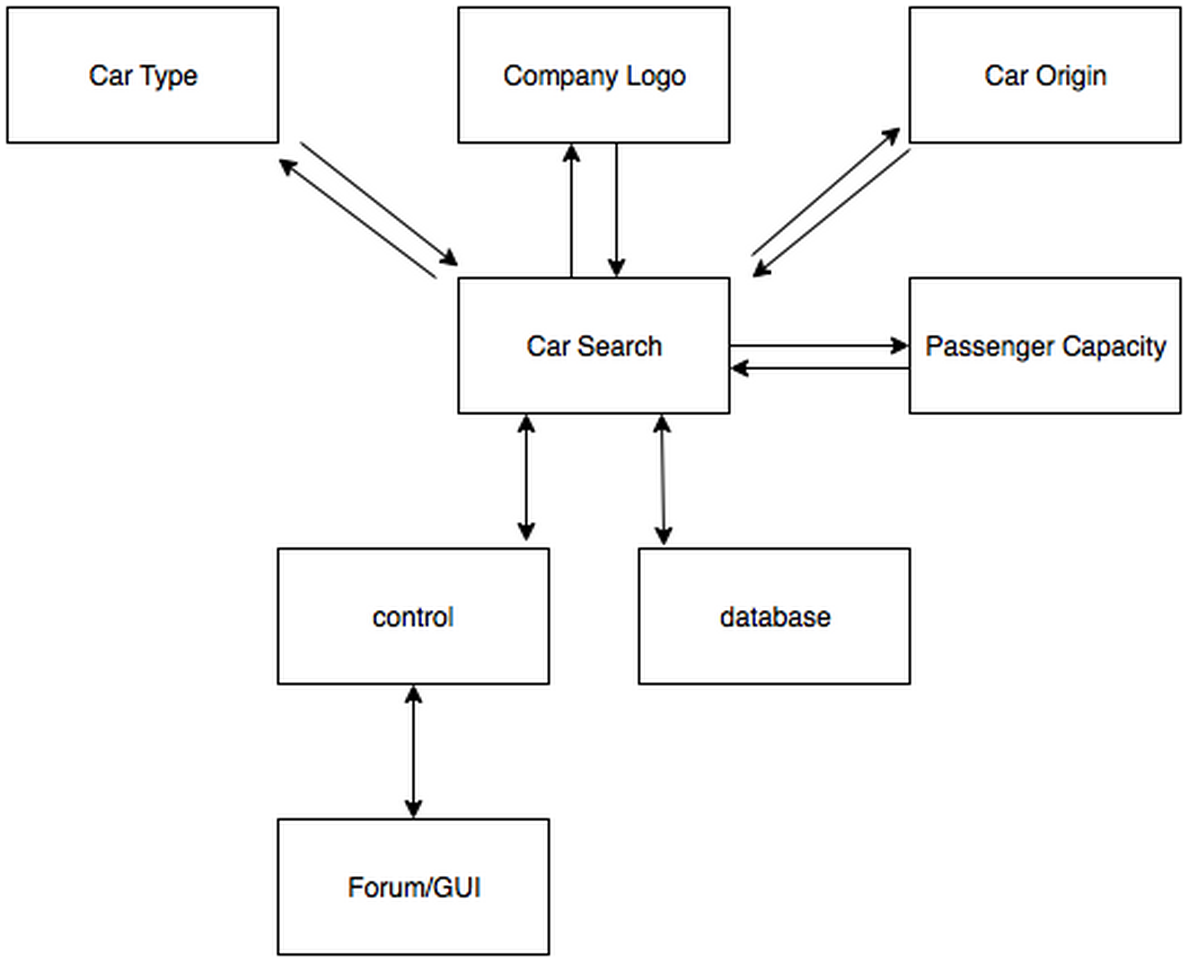
\includegraphics[width=\textwidth]{Structural.png}
\end{enumerate}
% End SubSection

\subsection{Subsystems}
\label{sub:subsystems}
% Begin SubSection
\begin{enumerate}[a)]
	\item {\textbf{Blackboard Subsystems}}
	\par Car Search:
	\par This subsystem uses car properties provided by the experts to find car models in the database which have the provided properties.
	\item {\textbf{Knowledge Source Subsystems}}
	\par Car Type:
	\par An expert which identifies the type of car (Sedan, SUV, Minivan, etc).
	\par Company Logo:
	\par An expert which identifies the company that made the car based on their logo.
	\par Car Origin:
	\par An expert which identifies the origin of the car (North American, European, etc).
	\par Passenger Capacity:
	\par An expert which identifies the number of passengers the car can hold.
	\par Database:
	\par A database containing car models and their properties. The database can be searched to find models which fit certain criteria.
	\item {\textbf{Controller Subsystem}}
	\par Control:
	\par This subsystem can initiate a car search and supervise the overall identification process.
\end{enumerate}
% End SubSection

% End Section
	
\section{Class Responsibility Collaboration (CRC) Cards}
\label{sec:class_responsibility_collaboration_crc_cards}
% Begin Section

	\begin{table}[ht]
		\centering
		\begin{tabular}{|p{5cm}|p{5cm}|}
		\hline 
		 \multicolumn{2}{|l|}{\textbf{Class Name:} CarDB} \\
		\hline
		\textbf{Responsibility:} & \textbf{Collaborators:} \\
		\hline
		Contain a listing of all car models and their attributes & -\\
		\hline
		Allow insertion and deletion of entries & -\\
		\hline
		Allow editing of entries & - \\
		\hline
		Provide information to CarSearchController & CarSearchController \\
		\hline
		\end{tabular}
	\end{table}
	
	\begin{table}[ht]
		\centering
		\begin{tabular}{|p{5cm}|p{5cm}|}
		\hline 
		 \multicolumn{2}{|l|}{\textbf{Class Name:} FeedbackStorage} \\
		\hline
		\textbf{Responsibility:} & \textbf{Collaborators:} \\
		\hline
		Contain a list of all feedback forms completed by users with anonymity, stored in a file & -\\
		\hline
	    Receive feedback from feedback form for storage & FeedbackForm\\
		\hline
		\end{tabular}
	\end{table}
	
	\begin{table}[ht]
		\centering
		\begin{tabular}{|p{5cm}|p{5cm}|}
		\hline 
		 \multicolumn{2}{|l|}{\textbf{Class Name:} FeedbackForm} \\
		\hline
		\textbf{Responsibility:} & \textbf{Collaborators:} \\
		\hline
	    Allow user to enter feedback about the application & -\\
		\hline
		\end{tabular}
	\end{table}
	
	\begin{table}[ht]
		\centering
		\begin{tabular}{|p{5cm}|p{5cm}|}
		\hline 
		 \multicolumn{2}{|l|}{\textbf{Class Name:} CarSearchController} \\
		\hline
		\textbf{Responsibility:} & \textbf{Collaborators:} \\
		\hline
		Contains algorithm to identify a car given some attributes & -\\
		\hline
	    Extract information from the SearchForm and compile it into a search query & SearchForm\\
	    \hline
	    Send result of search to SearchResult for display and verification & SearchResult\\
	    \hline
	    Query car database and experts as part of search algorithm to identify the car & CarDB, Expert\\
	    \hline
	    Control experts to be used in identification based on attributes given & ExpertPicker\\
		\hline
		\end{tabular}
	\end{table}

	\begin{table}[ht]
		\centering
		\begin{tabular}{|p{5cm}|p{5cm}|}
		\hline 
		 \multicolumn{2}{|l|}{\textbf{Class Name:} SearchResult} \\
		\hline
		\textbf{Responsibility:} & \textbf{Collaborators:} \\
		\hline
		Receive search result and send it to the forum to be displayed  & Forum,CarSearchController\\
		\hline
		Once a car identification is confirmed, result sent to search history & SearchHistory\\
		\hline
		Send result for verification before sending to search history & ResultVerifier\\
		\hline
		\end{tabular}
	\end{table}

	\begin{table}[ht]
		\centering
		\begin{tabular}{|p{5cm}|p{5cm}|}
		\hline 
		 \multicolumn{2}{|l|}{\textbf{Class Name:} ExpertPicker} \\
		\hline
		\textbf{Responsibility:} & \textbf{Collaborators:} \\
		\hline
		Control which experts will be used to identify the car based on attributes that are inputted & Expert\\
		\hline
		Set experts to "passive" or "active" for identification process & Expert\\
		\hline
		\end{tabular}
	\end{table}
	
	\begin{table}[ht]
		\centering
		\begin{tabular}{|p{5cm}|p{5cm}|}
			\hline 
			\multicolumn{2}{|l|}{\textbf{Class Name:} HelpPage} \\
			\hline
			\textbf{Responsibility:} & \textbf{Collaborators:} \\
			\hline
			Provide information about the application, and how to use it & -\\
			\hline
		\end{tabular}
	\end{table}

	\begin{table}[ht]
		\centering
		\begin{tabular}{|p{5cm}|p{5cm}|}
			\hline 
			\multicolumn{2}{|l|}{\textbf{Class Name:} Forum} \\
			\hline
			\textbf{Responsibility:} & \textbf{Collaborators:} \\
			\hline
			Central hub of application to allow navigation to various pages & SearchForm, SearchHistory, HelpPage, FeedbackForm\\
			\hline
			Display result of car identification & SearchResult\\
			\hline
		\end{tabular}
	\end{table}
	
	\begin{table}[ht]
		\centering
		\begin{tabular}{|p{5cm}|p{5cm}|}
			\hline 
			\multicolumn{2}{|l|}{\textbf{Class Name:} SearchForm} \\
			\hline
			\textbf{Responsibility:} & \textbf{Collaborators:} \\
			\hline
			Allow user to input characteristics of the car they want to identify & -\\
			\hline
			Send inputted attributes to car identification algorithm & CarSearchController\\
			\hline
		\end{tabular}
	\end{table}

	\begin{table}[ht]
		\centering
		\begin{tabular}{|p{5cm}|p{5cm}|}
			\hline 
			\multicolumn{2}{|l|}{\textbf{Class Name:} SearchHistory} \\
			\hline
			\textbf{Responsibility:} & \textbf{Collaborators:} \\
			\hline
			Store previous five confirmed identification results & -\\
			\hline
			When a new result enters the history, pushes out fifth most recent confirmed identification & -\\
			\hline
		\end{tabular}
	\end{table}

	\begin{table}[ht]
		\centering
		\begin{tabular}{|p{5cm}|p{5cm}|}
			\hline 
			\multicolumn{2}{|l|}{\textbf{Class Name:} DealershipLocator} \\
			\hline
			\textbf{Responsibility:} & \textbf{Collaborators:} \\
			\hline
			Interface with Google Maps API to locate dealerships that sell a specific car from the search history & SearchHistory\\
			\hline
		\end{tabular}
	\end{table}

	\begin{table}[ht]
		\centering
		\begin{tabular}{|p{5cm}|p{5cm}|}
			\hline 
			\multicolumn{2}{|l|}{\textbf{Class Name:} SecurityController} \\
			\hline
			\textbf{Responsibility:} & \textbf{Collaborators:} \\
			\hline
			Contains encryption and decryption mechanisms for transmitted messages & -\\
			\hline
			Decrypt search result once it arrives at the forum & Forum\\
			\hline
			Encrypt the search result before sending it to the forum & SearchResult\\
			\hline
		\end{tabular}
	\end{table}

	\begin{table}[ht]
		\centering
		\begin{tabular}{|p{5cm}|p{5cm}|}
			\hline 
			\multicolumn{2}{|l|}{\textbf{Class Name:} ResultVerifier} \\
			\hline
			\textbf{Responsibility:} & \textbf{Collaborators:} \\
			\hline
			Provide the user with the ability to confirm or deny the identified car result & -\\
			\hline
			Restart car identification if identified car is incorrect & CarSearchController\\
			\hline
			Restart search form if the identified car is incorrect three times & CarSearchController, SearchForm\\
			\hline
		\end{tabular}
	\end{table}

	\begin{table}[ht]
		\centering
		\begin{tabular}{|p{5cm}|p{5cm}|}
			\hline 
			\multicolumn{2}{|l|}{\textbf{Class Name:} Expert} \\
			\hline
			\textbf{Responsibility:} & \textbf{Collaborators:} \\
			\hline
			Know potential car identifications given certain attribute combinations in respective domain of expertise & -\\
			\hline
			Provide expertise to identify a car given some attributes of its domain & CarSearchController\\
			\hline
			Provide functionality to be set as "active" or "passive" when trying to identify a car & ExpertPicker\\
			\hline
		\end{tabular}
	\end{table}
% End Section

\FloatBarrier
\appendix
\section{Division of Labour}
\label{sec:division_of_labour}
% Begin Section
\begin{table}[ht]
	\centering
	\begin{tabular}{|p{5cm}|p{5cm}|}
		\hline 
		\textbf{Team Member:} & \textbf{Sections Completed:}\\
		\hline
		Abhijit & Section 1, 4\\
		\hline
		Cole & Section 3, 4, Reviewed and Reworked Business Events\\
		\hline
		David & Section 3, 5, Reviewed and Reworked Business Events\\
		\hline
		Sharon & Section 2, 3, Reviewed and Reworked Business Events\\
		\hline
		Yash & Section 3, 5, Reviewed and Reworked Business Events\\
		\hline
		Yuchen & Section 4\\
		\hline
	\end{tabular}
	\caption{Division of Labour}
	\label{table:1}
\end{table}
% End Section

\end{document}
%------------------------------------------------------------------------------